\documentclass[final]{beamer}

% ====================
% Packages
% ====================

\usepackage[T1]{fontenc}
\usepackage{lmodern}
\usepackage[orientation=portrait,size=a1,scale=1]{beamerposter}
\usetheme{gemini}
\usecolortheme{unito}
\usepackage{graphicx}
\usepackage{tikz}
\usepackage{pgfplots}
\pgfplotsset{compat=1.18}
\usepackage{anyfontsize}
\usepackage{multicol}
\usepackage{booktabs}
\usepackage{wrapfig}

% ====================
% Lengths
% ====================

\newlength{\sepwidth}
\newlength{\colwidth}
\setlength{\sepwidth}{0.001\paperwidth}
\setlength{\colwidth}{0.47\paperwidth}

\newcommand{\separatorcolumn}{\begin{column}{\sepwidth}\end{column}}

% ====================
% Title
% ====================

\title{Quantum-Classical Sentiment Analysis}
\author{Mario Bifulco\inst{1} \and Luca Roversi\inst{1}}
\institute[shortinst]{\inst{1} University of Turin, Computer Science Department}

% ====================
% Footer (optional)
% ====================

\footercontent{
  \raggedright
  \hspace{0.001\textwidth}
  \begin{minipage}[t]{0.1\textwidth}
    \raisebox{-0.68\height}{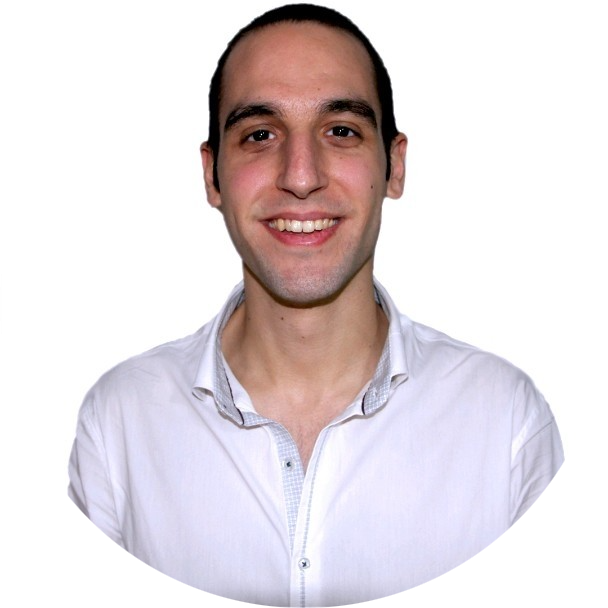
\includegraphics[width=\textwidth]{logos/circle.png}}
  \end{minipage}
  \hspace{0.01\textwidth}
  \begin{minipage}[t]{0.18\textwidth} 
    \small
    \textbf{Mario Bifulco} \\

    \textbf{Email:} \href{mario.bifulco@edu.unito.it}{mario.bifulco@edu.unito.it} \\
    \textbf{LinkedIn:} \href{https://www.linkedin.com/in/mario-bifulco/}{\url{linkedin.com/in/mario-bifulco/}} \\
    \textbf{GitHub:} \href{https://github.com/TheFlonet/qsvm4sentanalysis}{TheFlonet/qsvm4sentanalysis}
  \end{minipage}
  \hspace{0.01\textwidth}
  \begin{minipage}[t]{0.15\textwidth}
    \small 
    \textbf{Luca Roversi} \\

    \textbf{Email:} \href{luca.roversi@unito.it}{luca.roversi@unito.it} \\
    \textbf{Website:} \href{di.unito.it/~rover}{\url{di.unito.it/~rover}} \\
    \textbf{ORCID:} \href{https://orcid.org/0000-0002-1871-6109}{0000-0002-1871-6109}
  \end{minipage}
}

% ====================
% Logo (optional)
% ====================

\logoleft{
\includegraphics[height=3.5cm]{logos/logo-unito-orizz-neg.png}}
\logoright{
\includegraphics[height=3.5cm]{logos/EQAI-2024-logo.png}}

% ====================
% Body
% ====================

\begin{document}

\begin{frame}[t,fragile]
\begin{columns}[t]

\begin{column}{\colwidth}
  \begin{block}{Abstract}
    We first experiment with applying a hybrid classical-adiabatic quantum classifier (HCAQC) for sentiment analysis and compare it to the classical classifier and state-of-the-art Transformer architecture. 
    HCAQC is worse than Transformer in classification, but it converges to a good solution much more quickly. 
    Secondly, the work explores how to address a bottleneck of HCAQC. 
    The results show how effective HCAQCs can be developed, making greater use of the quantum component.
  \end{block}

  \begin{block}{Quantum Support Vector Machine for Sentiment Analysis}
    We explore the potential of \textbf{Adiabatic Quantum Computing (AQC)} for \textbf{Natural Language Processing (NLP)}. The focus is on \textbf{Binary Sentiment Analysis (BSA)}. 
    Our steps are:

    \begin{enumerate} 
        \item Select the TweetEval dataset\cite{TweetEval}; 
        \item Transform the text into vectors using SentenceBert\cite{SentenceBert}; 
        \item Encode the problem of learning a \textbf{Support Vector Machine (SVM)} using the D-Wave hybrid solvers; 
        \item Assess the quality. We compare it with:
        \begin{itemize}
            \item An SVM implementation via CPLEX classical solver;
            \item The Transformer RoBERTa\cite{roberta}.
        \end{itemize} 
    \end{enumerate}
\end{block}

  \begin{block}{QSVM Results}
    Legend of labels: \textbf{D-Wave} represents the quantum solution, \textbf{CPLEX} represents the classical implementation of SVM, \textbf{RoBERTa} represents the Transformer architecture.

    \begin{figure}[h!]
        \centering
        \begin{minipage}{0.3\textwidth}
            \centering
            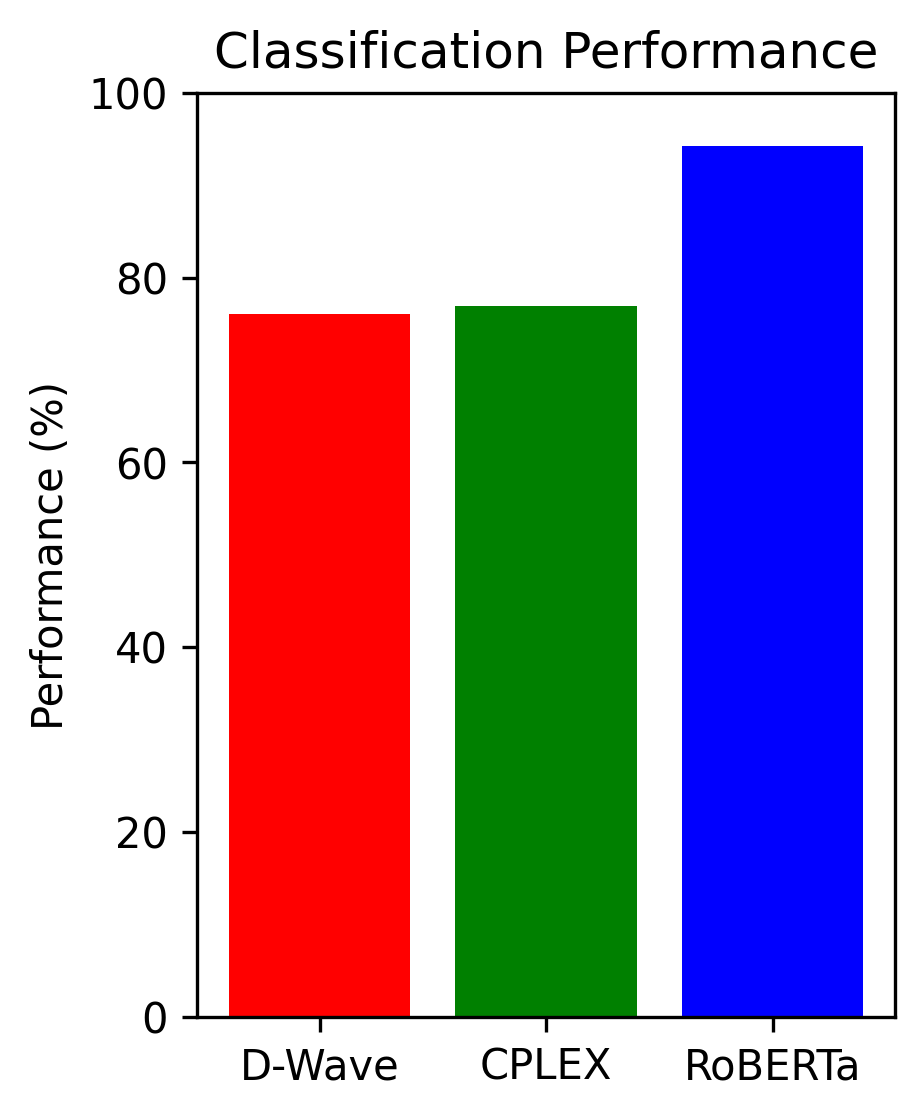
\includegraphics[height=0.14\textheight]{logos/performance.png}
        \end{minipage}%
        \hfill
        \begin{minipage}{0.65\textwidth}
            \begin{alertblock}{Classification Performance}
                RoBERTa is almost 20\% better than D-Wave and CPLEX, which classify 75\% of cases correctly.
            
                CPLEX is slightly better than D-Wave due to some limitations of the current hybrid solvers, which restrict the domain of the optimisation variables from real numbers to integers.
            \end{alertblock}
        \end{minipage}
    \end{figure}

    \begin{figure}[h!]
        \centering
        \begin{minipage}{0.65\textwidth}
            \begin{alertblock}{Training Time}
                The time required by D-Wave to find an optimal assignment is 60\% less than that of CPLEX. 

                Although not available, it is reasonable to expect an even better result if compared to the time required by RoBERTa, which we can fairly expect to amount to several hours of training on high-performance machines.
            \end{alertblock}
        \end{minipage}%
        \hfill
        \begin{minipage}{0.3\textwidth}
            \centering
            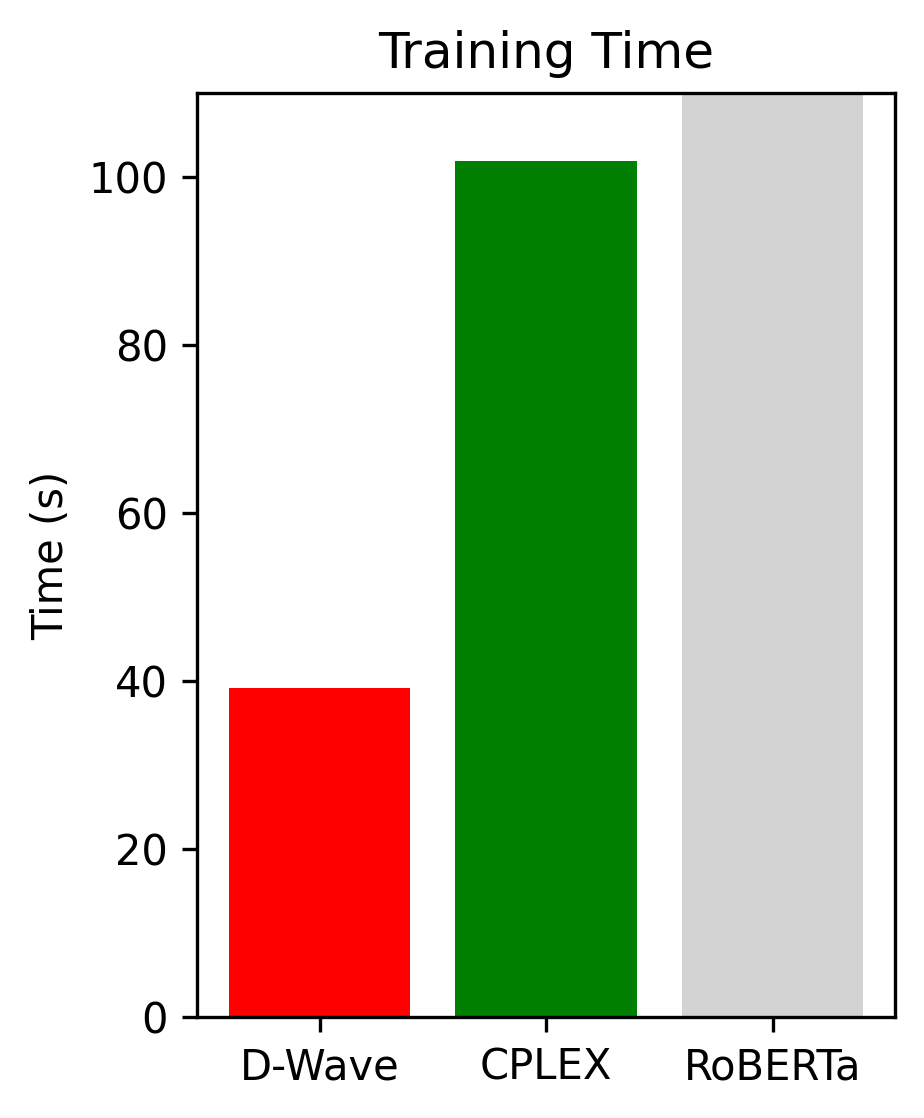
\includegraphics[height=0.14\textheight]{logos/training.png}
        \end{minipage}
    \end{figure}

    \begin{figure}[h!]
        \centering
        \begin{minipage}{0.3\textwidth}
            \centering
            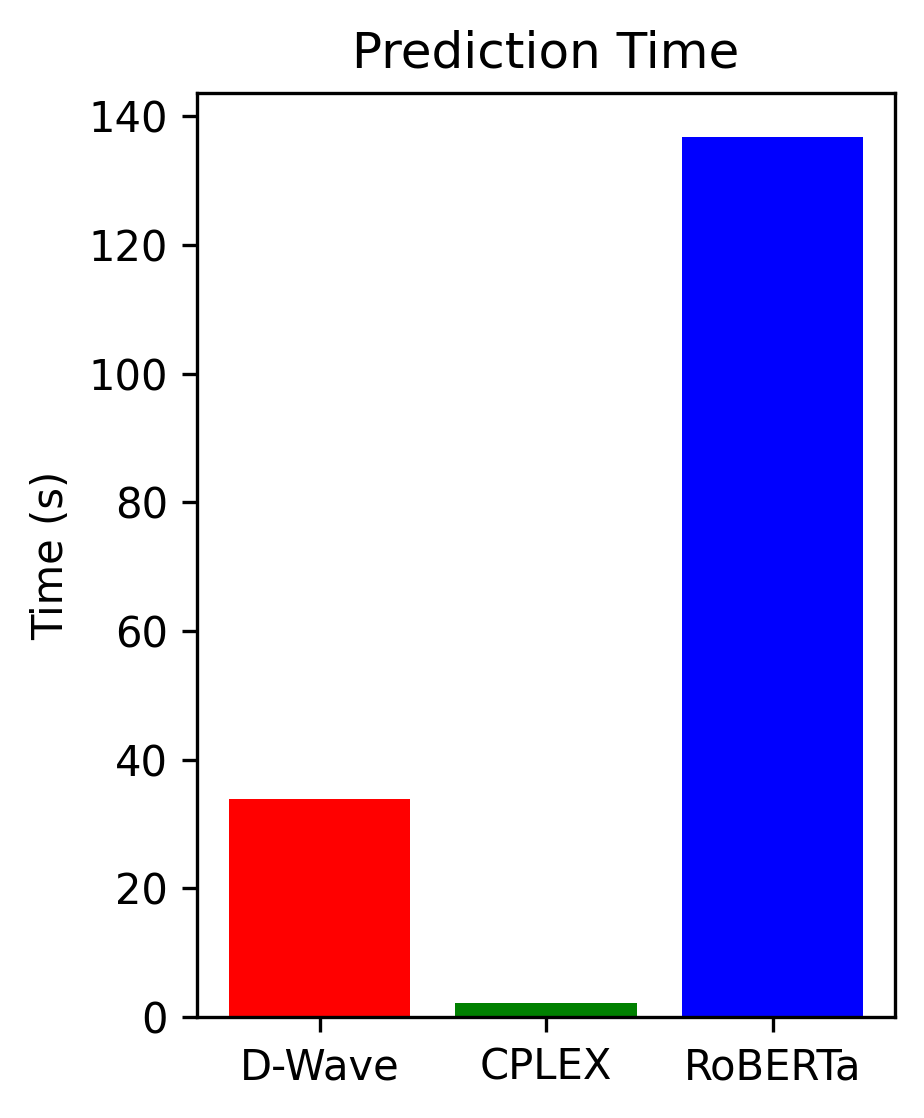
\includegraphics[height=0.14\textheight]{logos/prediction.png}
        \end{minipage}%
        \hfill
        \begin{minipage}{0.65\textwidth}
            \begin{alertblock}{Prediction Time}
                The complexity of the RoBERTa architecture also affects the time required for prediction.

                The longer time D-Wave requires is due to the resolution methodology, which returns a set of optimal solutions from which a majority vote is taken during inference.

                Experimentally, we find that it is possible to use only the first of the optimal assignments produced, reducing the time to values comparable to those of CPLEX.
            \end{alertblock}
        \end{minipage}
    \end{figure}
\end{block}

  \begin{block}{Maximizing Quantum Boost} 
    Experiments show that the D-Wave solver makes marginal use of the QPU: average contribution of \textbf{0.08\%}. 
    For greater performance, we run the problem directly on the QPU: bypass the opaque workflow D-Wave proprietary technology hybrid solvers.
   
    We transform the learning of an SVM into a problem that is solvable directly by the QPU. Among the series of required steps, the only one impacting performance is the calculation of a minor embedding\cite{MEdwave}.
   
    \begin{figure}[h!]
        \centering
        \begin{minipage}{0.55\textwidth}
        \begin{alertblock}{QPU Bottleneck}
            Empirically, we identify a sweet spot for problems with 32 variables.
                        
            Beyond this size, the time required to find the minor graph can become dominant compared to the time needed to solve the problem.

            Additionally, the number of qubits required to represent the problem graph becomes incompatible with the current QPU sizes (approximately 5600 qubits).
        \end{alertblock}
        \end{minipage}%
        \hfill
        \begin{minipage}{0.4\textwidth}
            \centering
            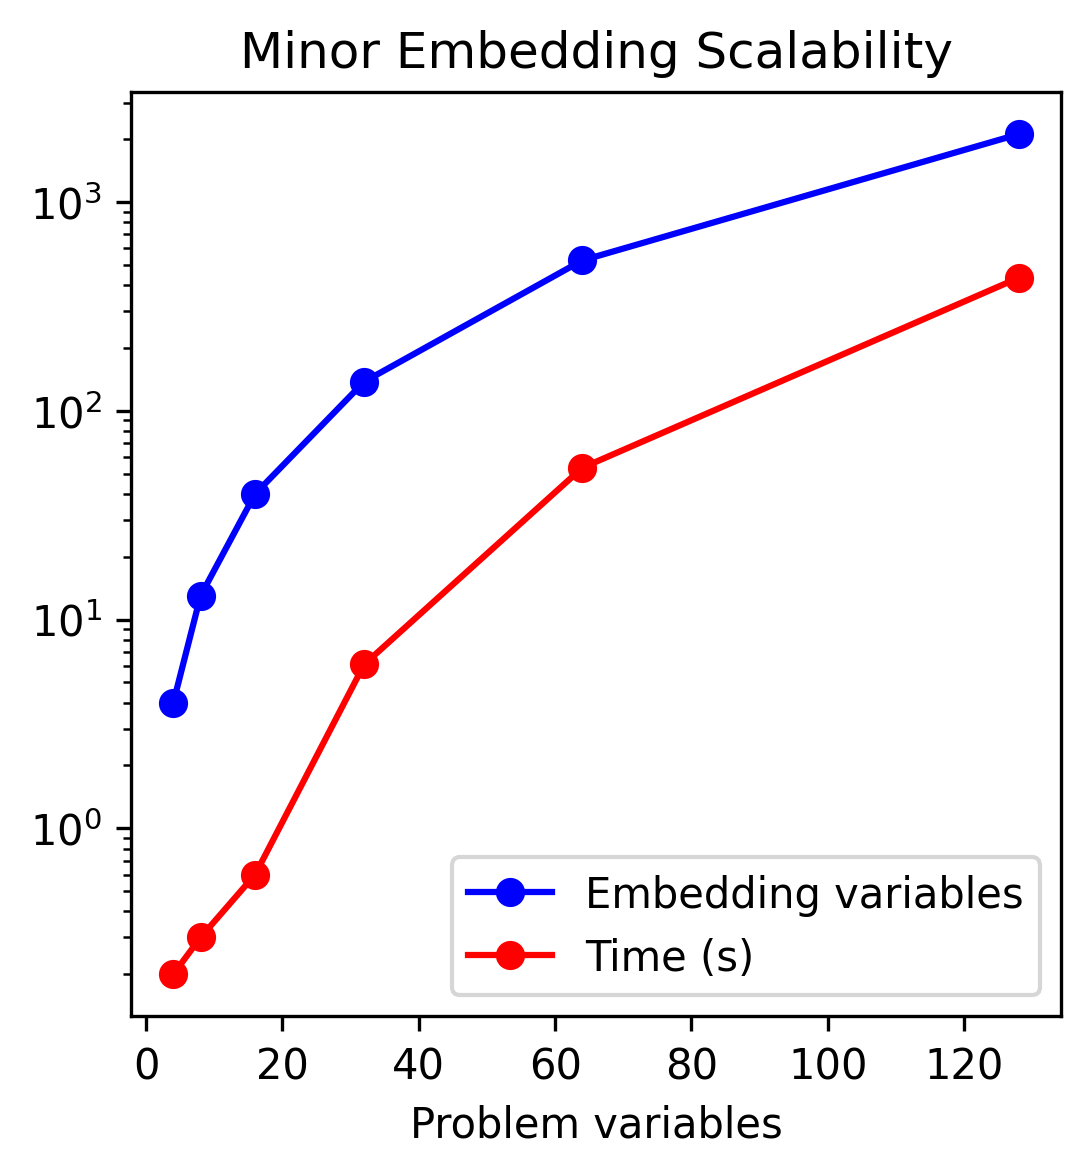
\includegraphics[height=0.14\textheight]{logos/embedding_search_time.png}
        \end{minipage}
    \end{figure}
\end{block}
\end{column}

\separatorcolumn

\begin{column}{\colwidth}
  \begin{block}{Homebrewing a Hybrid Solver}
    We design \texttt{QSplit}, a hybrid solver to increase the usage time of QPU.
    \texttt{QSplit} decomposes a QUBO problem into smaller QUBOS.
    \texttt{QSplit} relies on simple algebraic properties.

    \begin{figure}[h!]
        \centering
        \begin{minipage}{0.55\textwidth}
            Given any QUBO matrix we recursively divide it into four parts as in Figure \ref{fig:qubo}:
            \begin{enumerate}
                \item $\operatorname{ULs}$ and $\operatorname{BRs}$ are themselves QUBO matrices operating on a partition of the optimization variables;
                \item $\operatorname{UR}$ retains the information linking the partitions $\operatorname{UL}_0$ and $\operatorname{BR}_0$ of the variables and we can safely transform it into an upper triangular matrix, namely a QUBO instance;
                \item $\emptyset$ is a matrix composed entirely of zeros, so we ignore it.
            \end{enumerate}

            The recursive subdivision can continue until the matrices reach a predetermined size, namely the Stopping dimension.
        \end{minipage}%
        \hfill
        \begin{minipage}{0.4\textwidth}
            \centering
            \begin{tikzpicture}
                \draw (0,0) rectangle (8,8);
            
                \draw (0,4) -- (8,4);
                \draw (4,0) -- (4,8);
                \node at (2,2) {$\emptyset$};
                
                \draw (0,6) -- (4,6);
                \draw (2,8) -- (2,4);
                \node at (1,5) {$\emptyset$};
            
                \draw (4,2) -- (8,2);
                \draw (6,4) -- (6,0);
                \node at (5,1) {$\emptyset$};

                \draw (4,6) -- (8,6);
                \draw (6,4) -- (6,8);
                \node at (5,5) {$\emptyset$};
            
                \draw[decorate,decoration={brace,amplitude=10pt}] (8,8) -- (8,4) node [black,midway,xshift=25pt] {$\operatorname{UR}_0$};
                \node at (3,7) {$\operatorname{UR}_1'$};
                \node at (7,7) {$\operatorname{UR}_1''$};
                \node at (7,3) {$\operatorname{UR}_1'''$};

                \draw[decorate,decoration={brace,amplitude=10pt,mirror}] (0,8) -- (0,4) node [black,midway,xshift=-25pt] {$\operatorname{UL}_0$};
                \node at (1,7) {$\operatorname{UL}_1'$};
                \node at (5,7) {$\operatorname{UL}_1''$};
                \node at (5,3) {$\operatorname{UL}_1'''$};

                \draw[decorate,decoration={brace,amplitude=10pt}] (8,4) -- (8,0) node [black,midway,xshift=25pt] {$\operatorname{BR}_0$};
                \node at (3,5) {$\operatorname{BR}_1'$};
                \node at (7,5) {$\operatorname{BR}_1''$};
                \node at (7,1) {$\operatorname{BR}_1'''$};

                \draw[decorate,decoration={brace,amplitude=10pt,mirror}] (0,4) -- (0,0) node [black,midway,xshift=-25pt] {$\operatorname{BL}_0$};
            \end{tikzpicture}
            \caption{Two steps of recursive decomposition}
            \label{fig:qubo}
        \end{minipage}
    \end{figure}

    \begin{exampleblock}{Example of one recursive step}
        Let us assume that we have classifications offered by $\operatorname{UL}_1'$, $\operatorname{UR}_1'$, $\operatorname{BR}_1'$. 

        \begin{enumerate}
            \item $\operatorname{UL}_1'$ and $\operatorname{BR}_1'$ are combined to generate conflict-free initial assignments called $\operatorname{S_1}$;
            \item The solutions from $\operatorname{S_1}$ and $\operatorname{UR}_1'$ are combined, and conflicting variables are marked;
            \item From the conflicting values, a QUBO problem is extracted, which is solved via QPU;
            \item From the set of possible assignments, the $k$ best distinct assignments are retained. 
        \end{enumerate}
    \end{exampleblock}
\end{block}

  \begin{block}{\texttt{QSplit} Results}
    We tested \texttt{QSplit} with problems from 128 variables, and the data collected showed the following behaviour \textbf{when decreasing the Stopping dimension}.

    \begin{figure}[h!]
        \centering
        \begin{minipage}{0.55\textwidth}
            \centering
            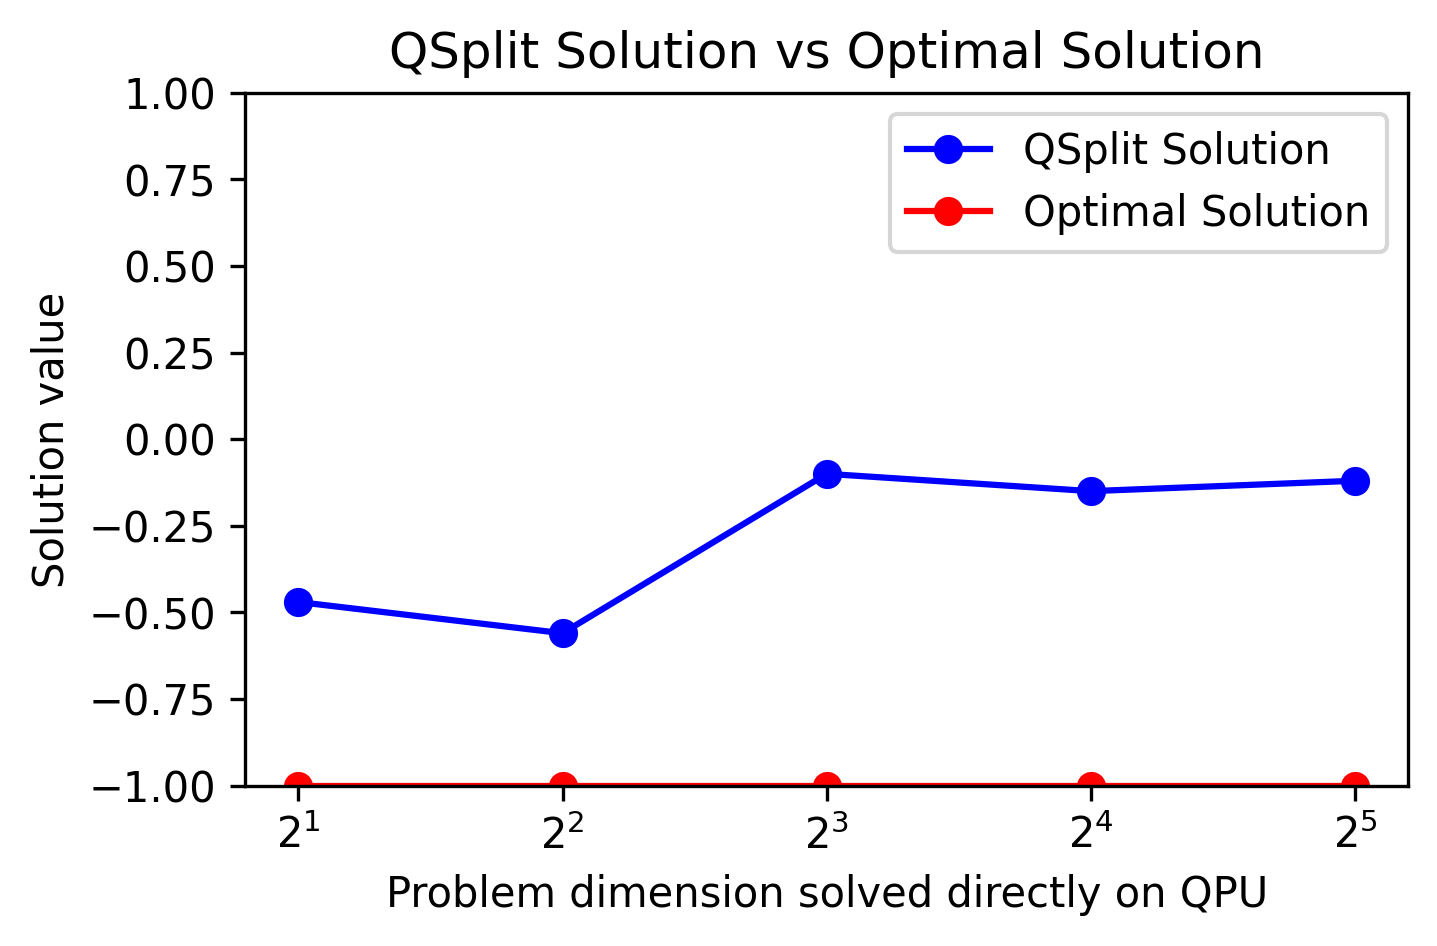
\includegraphics[height=0.14\textheight]{logos/sol.png}
        \end{minipage}%
        \hfill
        \begin{minipage}{0.4\textwidth}
            \begin{alertblock}{Performance}
                The quality of the solution improves, with the error decreasing from 45\% to 25\%.
            \end{alertblock}
        \end{minipage}
    \end{figure}

    \begin{figure}[h!]
        \centering
        \begin{minipage}{0.4\textwidth}
            \begin{alertblock}{Execution Time}
                The time required by \texttt{QSplit} increases, ranging from requiring 40\% less time compared to direct resolution to requiring 50\% more time.
            \end{alertblock}
        \end{minipage}%
        \hfill
        \begin{minipage}{0.55\textwidth}
            \centering
            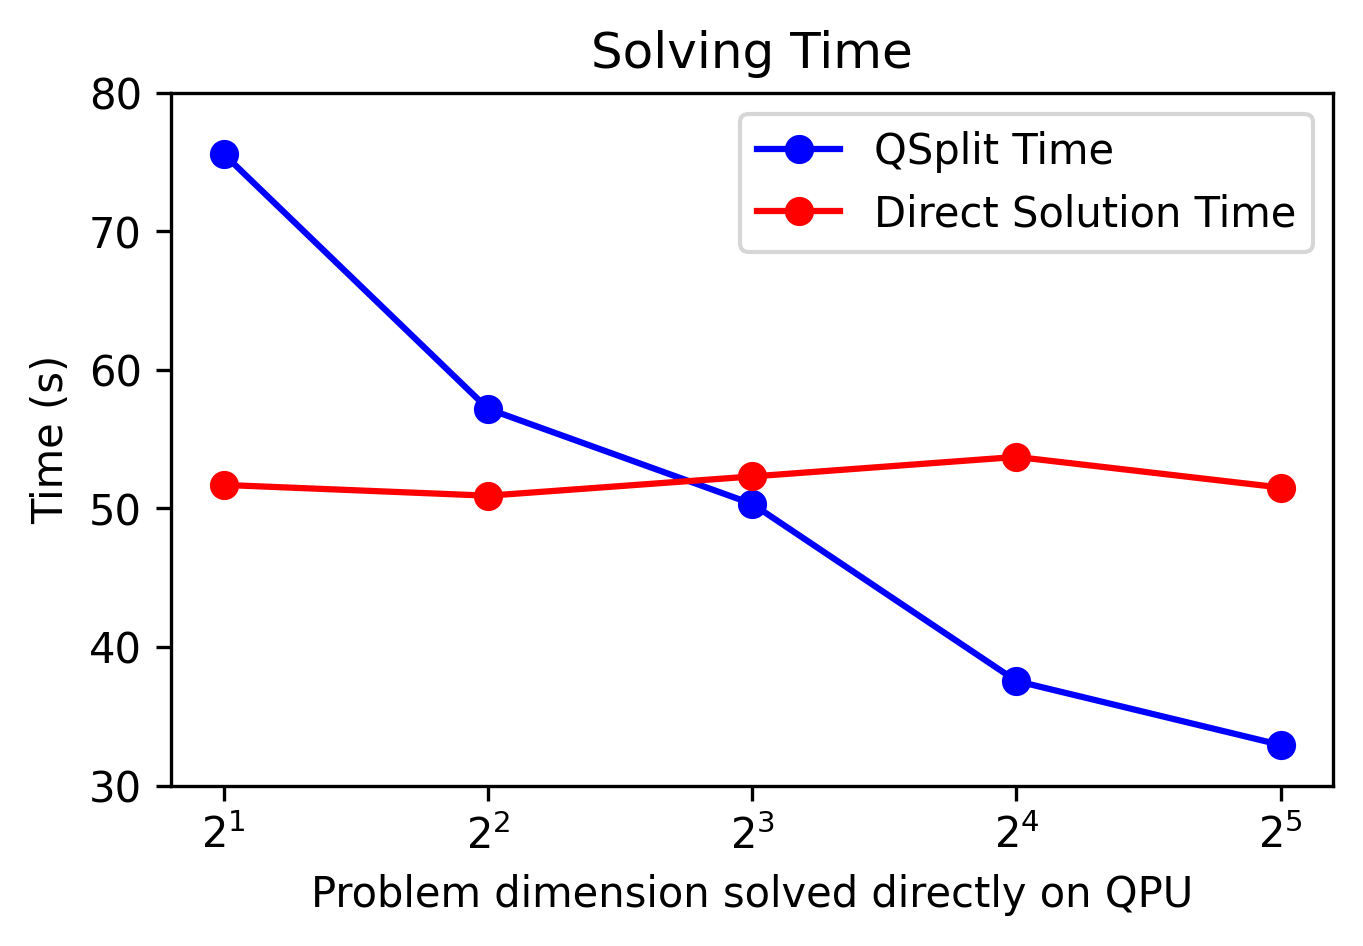
\includegraphics[height=0.14\textheight]{logos/time.png}
        \end{minipage}
    \end{figure}
\end{block}

  \begin{block}{Conclusion}
    We give evidence that quantum computing can bring tangible benefits over traditional methods to solve optimization problems.
    It is useful because:
    \begin{itemize}
      \item Converges much faster to the solution than classical methods;
      \item Requires limited hardware resources, allowing it to be used in embedded systems and personal computers.
    \end{itemize} 

    \texttt{QSplit} is an experimental solution for handling large QUBO problems, different from those found in the literature\cite{subqubo2}. 
    The assignment produced can be improved by implementing more refined problem partitioning strategies\cite{bnb}, or by creating work pipelines capable of using a set of methods for finding the optimal assignment\cite{dwavehybrid}.
  \end{block}

  \begin{block}{Bibliography}
    \begin{thebibliography}{10}
      \bibitem{TweetEval} Rosenthal Sara et al., ``SemEval-2017 task 4: Sentiment analysis in Twitter''.
      \bibitem{SentenceBert} Reimers Nils et al., ``Sentence-BERT: Sentence Embeddings using Siamese BERT-Networks''.
      \bibitem{roberta} CardiffNLP, ``Twitter-roBERTa-base for Sentiment Analysis''.
      \bibitem{MEdwave} Jun Cai et al., ``A practical heuristic for finding graph minors''.
      \bibitem{subqubo2} Tameem Albash et al., ``Solving large optimization problems with restricted quantum annealers''.
      \bibitem{bnb} Sanavio Claudio et al., ``Hybrid Classical–Quantum Branch-and-Bound Algorithm for Solving Integer Linear Problems''.
      \bibitem{dwavehybrid} Michael Booth et al., ``Partitioning Optimization Problems for Hybrid Classical/Quantum Execution''.
    \end{thebibliography}
  \end{block}
\end{column}

\end{columns}
\end{frame}

\end{document}
